\documentclass[12pt,a4paper]{article}

\usepackage[utf8]{inputenc}
\usepackage[T1]{fontenc}
\usepackage[spanish,es-nodecimaldot]{babel}
\usepackage{graphicx}
\usepackage{geometry}
\geometry{top=2.5cm,bottom=2.5cm,left=2.5cm,right=2.5cm}
\usepackage{xcolor}
\usepackage{hyperref}
\usepackage{longtable}
\usepackage{tabularx}
\usepackage{booktabs}
\usepackage{listings}
\usepackage{fancyhdr}
\usepackage{tcolorbox}
\usepackage{titlesec}
\usepackage{enumitem}
\usepackage{caption}
\usepackage{amsmath}

% Colores institucionales y de código
\definecolor{unsaacblue}{RGB}{0, 51, 102}
\definecolor{darkblue}{RGB}{10, 40, 95}
\definecolor{accentblue}{RGB}{25, 118, 210}
\definecolor{codegreen}{RGB}{46, 125, 50}
\definecolor{codegray}{RGB}{100, 116, 139}
\definecolor{codepurple}{RGB}{124, 58, 237}
\definecolor{backcolour}{RGB}{248, 250, 252}
\definecolor{bordercolor}{RGB}{226, 232, 240}
\definecolor{calloutbg}{RGB}{240, 249, 255}
\definecolor{calloutborder}{RGB}{56, 189, 248}

% Configuración de listings para código Dart / Flutter
\lstdefinelanguage{Dart}{
  morekeywords={
    abstract,as,assert,async,await,break,case,catch,class,const,continue,
    default,deferred,do,dynamic,else,enum,export,extends,external,factory,
    false,final,finally,for,Function,get,hide,if,implements,import,in,
    interface,is,late,library,mixin,new,null,of,on,operator,part,rethrow,
    return,set,show,static,super,switch,sync,this,throw,true,try,typedef,
    var,void,while,with,yield,override,required
  },
  morecomment=[l]{//},
  morecomment=[s]{/*}{*/},
  morestring=[b]',
  morestring=[b]",
  sensitive=true
}

\lstset{
  language=Dart,
  backgroundcolor=\color{backcolour},
  commentstyle=\color{codegreen}\itshape,
  keywordstyle=\color{unsaacblue}\bfseries,
  numberstyle=\tiny\color{codegray},
  stringstyle=\color{codepurple},
  basicstyle=\ttfamily\footnotesize,
  breakatwhitespace=false,
  breaklines=true,
  captionpos=b,
  keepspaces=true,
  numbers=left,
  numbersep=7pt,
  showspaces=false,
  showstringspaces=false,
  showtabs=false,
  tabsize=2,
  frame=single,
  rulecolor=\color{bordercolor},
  xleftmargin=15pt,
  framexleftmargin=15pt
}

\hypersetup{
  colorlinks=true,
  linkcolor=unsaacblue,
  filecolor=magenta,
  urlcolor=accentblue,
  citecolor=unsaacblue
}

% Encabezados y pies de página
\pagestyle{fancy}
\fancyhf{}
\fancyhead[L]{\small\color{codegray}UNSAAC - Desarrollo de Software II}
\fancyhead[R]{\small\color{codegray}Práctica 04: Widgets en Flutter}
\fancyfoot[C]{\thepage}
\renewcommand{\headrulewidth}{0.4pt}
\renewcommand{\footrulewidth}{0.4pt}

\begin{document}

% ==============================================================================
% CARÁTULA OFICIAL INSTITUCIONAL UNSAAC
% ==============================================================================
\begin{titlepage}
    \centering
    {\bfseries\large UNIVERSIDAD NACIONAL DE SAN ANTONIO ABAD DEL CUSCO\par}
    \vspace{0.2cm}
    {\bfseries\normalsize FACULTAD DE INGENIERÍA ELÉCTRICA, ELECTRÓNICA, INFORMÁTICA Y MECÁNICA\par}
    \vspace{0.2cm}
    {\bfseries\normalsize ESCUELA PROFESIONAL DE INGENIERÍA INFORMÁTICA Y DE SISTEMAS\par}
    \vspace{0.8cm}
    
\includegraphics[width=0.35\textwidth]{unsaac.jpg}\par
    \vspace{0.8cm}
    {\Large\bfseries ASIGNATURA: DESARROLLO DE SOFTWARE II\par}
    \vspace{0.4cm}
    {\large\bfseries TRABAJO: PRÁCTICA 04: GUÍA PRÁCTICA DE WIDGETS EN FLUTTER\par}
    \vspace{0.4cm}
    {\large\bfseries REFERENCIA COMPLETA, CATÁLOGO INTERACTIVO Y APLICACIÓN DE DEMOSTRACIÓN DE WIDGETS\par}
    \vspace{1.2cm}
    \begin{flushleft}
    \textbf{DOCENTE RESPONSABLE:} \\
    Ing. Hans Harley Ccacyahuillca Bejar\\[0.5cm]
    \textbf{AUTOR / DESARROLLADOR:} \\
    SUPA CUSIPAUCAR, Yeferson - 220553\\[0.5cm]
    \textbf{SEMESTRE ACADÉMICO:} \\
    2026-II (Décimo Semestre)\\[0.5cm]
    \textbf{REPOSITORIO OFICIAL:} \\
    \url{https://github.com/YefersonSupa/Desarrollo_SoftwareII}
    \end{flushleft}
    \vfill
    {\bfseries\large Cusco - Perú\par}
    {\bfseries 2026\par}
\end{titlepage}

\tableofcontents
\newpage

% ==============================================================================
% 1. INFORMACIÓN GENERAL Y FICHA TÉCNICA
% ==============================================================================
\section{Información General del Proyecto}

El presente informe técnico documenta el desarrollo de la \textbf{Práctica N$^\circ$ 4: Guía Práctica de Widgets en Flutter} de la asignatura \textbf{Desarrollo de Software II}. En esta práctica se analiza y desarrolla una aplicación móvil interactiva y modular construida con Flutter 3.47 y Dart 3.13 que cubre 25 widgets distribuidos en cinco categorías arquitectónicas: \textit{Layout}, \textit{Display}, \textit{Input}, \textit{Navegación} y \textit{Feedback}.

\begin{tcolorbox}[colback=calloutbg,colframe=calloutborder,title=\textbf{Ficha Técnica de la Práctica 04}]
\textbf{Institución:} Universidad Nacional de San Antonio Abad del Cusco (UNSAAC)\\
\textbf{Escuela Profesional:} Ingeniería Informática y de Sistemas\\
\textbf{Asignatura:} Desarrollo de Software II\\
\textbf{Docente:} Ing. Hans Harley Ccacyahuillca Bejar\\
\textbf{Estudiante:} SUPA CUSIPAUCAR, Yeferson (Código: 220553)\\
\textbf{Entorno de Desarrollo:} Flutter SDK 3.47.4, Dart SDK 3.13.3, Android SDK 36.0.0\\
\textbf{Ubicación del Código:} \texttt{/lab\_04/widgets\_app}\\
\textbf{Repositorio en GitHub:} \url{https://github.com/YefersonSupa/Desarrollo_SoftwareII}
\end{tcolorbox}

% ==============================================================================
% 2. FUNDAMENTOS DE LA ARQUITECTURA DE WIDGETS EN FLUTTER
% ==============================================================================
\section{Fundamentos de la Arquitectura de Widgets en Flutter}

\subsection{¿Qué es un Widget en Flutter?}
En Flutter, el paradigma rector es declarativo: \textbf{"Todo es un widget"}. A diferencia de los marcos de trabajo imperativos donde las vistas mutan directamente en memoria, un widget en Flutter es una descripción inmutable (\textit{blueprint}) de una parte de la interfaz de usuario. Los widgets describen cómo debe lucir la UI dado un estado y configuración específicos.

\subsection{El Modelo de Tres Árboles (Three Trees)}
Para comprender el rendimiento a 60/120 FPS de Flutter, es necesario comprender la interacción entre los tres árboles paralelos:
\begin{enumerate}[leftmargin=*]
    \item \textbf{Widget Tree (Árbol de Widgets):} Estructura jerárquica de configuración inmutable y de corta vida. Se crea y destruye con bajo costo computacional cada vez que el estado cambia.
    \item \textbf{Element Tree (Árbol de Elementos):} Estructura persistente que representa la instanciación real en memoria del widget en el árbol. Vincula el widget conceptual con el objeto gráfico subyacente y almacena el estado en los \texttt{StatefulWidgets}.
    \item \textbf{RenderObject Tree (Árbol de Objetos de Renderizado):} Nodos de bajo nivel que gestionan el cálculo de geometría, restricciones espaciales (\textit{constraints}), maquetación (\textit{layout}) y pintado (\textit{paint}) directo sobre el lienzo (\textit{canvas}) mediante el motor Skia/Impeller.
\end{enumerate}

\subsection{El Punto de Entrada: main() y runApp()}
Toda aplicación Flutter inicia en la función canónica de Dart \texttt{main()}, delegando la inicialización del motor a \texttt{runApp()}:

\begin{lstlisting}[caption={Punto de entrada de una aplicación Flutter},label={lst:main}]
void main() {
  // Infla el widget raiz y lo enlaza al RenderView de la pantalla
  runApp(const WidgetsGuideApp());
}
\end{lstlisting}

\begin{itemize}[leftmargin=*]
    \item \texttt{void main()}: Función de entrada estándar requerida por el compilador de Dart.
    \item \texttt{runApp()}: Inicializa los bindings del framework (\texttt{WidgetsBinding}), infla el widget raíz y lo conecta al sistema de ventanas del sistema operativo.
    \item \texttt{const}: Indica inmutabilidad en tiempo de compilación, evitando reconstrucciones redundantes en ciclos subsiguientes.
\end{itemize}

\subsection{StatelessWidget vs. StatefulWidget y BuildContext}
\begin{itemize}[leftmargin=*]
    \item \textbf{StatelessWidget:} Empleado para interfaces cuya presentación no depende de un estado mutable que cambie durante la vida útil del widget (ej. iconos, textos estáticos).
    \item \textbf{StatefulWidget:} Compuesto por dos clases: la configuración inmutable (\texttt{StatefulWidget}) y el contenedor de estado mutable (\texttt{State<T>}). Al ejecutar \texttt{setState()}, se planifica una llamada al método \texttt{build()} para reconciliar la vista.
    \item \textbf{BuildContext:} Manejador que localiza la posición relativa del widget dentro del \textit{Element Tree}. Permite acceder a recursos heredados como temas (\texttt{Theme.of(context)}) y dimensiones (\texttt{MediaQuery.of(context)}).
\end{itemize}

\subsection{Configuración Global con MaterialApp y Scaffold}
\begin{lstlisting}[caption={Configuración global con MaterialApp y Scaffold},label={lst:materialapp}]
return MaterialApp(
  title: 'Guia Practica de Widgets en Flutter',
  theme: ThemeData(
    colorScheme: ColorScheme.fromSeed(
      seedColor: const Color(0xFF5E35B1),
      brightness: Brightness.light,
    ),
    useMaterial3: true,
  ),
  home: const HomeScreen(),
);
\end{lstlisting}

\begin{itemize}[leftmargin=*]
    \item \texttt{MaterialApp}: Provee servicios de diseño Material 3, enrutamiento, localización e inyección de temas.
    \item \texttt{ThemeData}: Centraliza los tokens de diseño (tipografías, colores, formas). \texttt{ColorScheme.fromSeed} genera una paleta cromática armónica a partir de un color semilla.
    \item \texttt{Scaffold}: Estructura visual estándar que ofrece slots para \texttt{appBar}, \texttt{body}, \texttt{floatingActionButton}, \texttt{drawer} y \texttt{bottomNavigationBar}.
\end{itemize}

% ==============================================================================
% 3. CATÁLOGO COMPLETO DE LOS 25 WIDGETS
% ==============================================================================
\section{Catálogo Técnico de los 25 Widgets Desarrollados}

A continuación, se resume la matriz de los 25 widgets implementados en la aplicación interactiva:

\begin{small}
\begin{longtable}{|p{0.8cm}|p{2.2cm}|p{2.3cm}|p{5.5cm}|p{3.5cm}|}
\caption{Matriz técnica completa de los 25 widgets desarrollados en la práctica.} \label{tab:widgets_completa} \\
\hline
\textbf{\#} & \textbf{Categoría} & \textbf{Widget} & \textbf{Propósito y Descripción} & \textbf{Propiedades Clave} \\
\hline
\endfirsthead
\multicolumn{5}{c}%
{{\bfseries \tablename\ \thetable{} -- Continuación de la página anterior}} \\
\hline
\textbf{\#} & \textbf{Categoría} & \textbf{Widget} & \textbf{Propósito y Descripción} & \textbf{Propiedades Clave} \\
\hline
\endhead
\hline \multicolumn{5}{|r|}{{Continúa en la siguiente página...}} \\ \hline
\endfoot
\hline
\endlastfoot

1 & Layout & Container & Caja con margen, padding, bordes redondeados y dimensiones. & width, height, padding, margin, decoration, child \\ \hline
2 & Layout & Row & Alinea elementos secuencialmente en el eje horizontal. & mainAxisAlignment, crossAxisAlignment, children \\ \hline
3 & Layout & Column & Alinea elementos secuencialmente en el eje vertical. & mainAxisAlignment, crossAxisAlignment, mainAxisSize \\ \hline
4 & Layout & Stack & Superpone widgets en capas en el eje Z mediante coordenadas. & alignment, fit, children, Positioned \\ \hline
5 & Layout & Expanded / Flexible & Distribuyen proporcionalmente el espacio restante con flex. & flex, fit, child \\ \hline
6 & Layout & Padding / SizedBox & Control de espaciado interno y separadores dimensionales. & padding, width, height, child \\ \hline
7 & Display & Text & Renderizado tipográfico avanzado y truncamiento. & style, maxLines, overflow, textAlign \\ \hline
8 & Display & Image & Carga de imágenes locales, remotas y control de ajuste. & fit, width, height, alignment \\ \hline
9 & Display & Card & Superficie elevada con sombra material y bordes circulares. & elevation, shape, color, child, margin \\ \hline
10 & Display & CircleAvatar & Avatar circular con imagen de fondo o iniciales fallback. & radius, backgroundImage, backgroundColor \\ \hline
11 & Display & ListView & Lista desplazable eficiente con reciclado de memoria. & itemCount, itemBuilder, scrollDirection \\ \hline
12 & Display & GridView & Matriz bidimensional en cuadrícula con delegados de rejilla. & gridDelegate, itemCount, itemBuilder \\ \hline
13 & Input & ElevatedButton & Botón material elevado para acciones prioritarias. & onPressed, style, child \\ \hline
14 & Input & TextField & Captura y validación de texto editable con controladores. & controller, decoration, keyboardType \\ \hline
15 & Input & Switch / Checkbox & Selección y alternancia de variables booleanas de configuración. & value, onChanged, activeColor \\ \hline
16 & Input & DropdownButton & Selector de lista desplegable fuertemente tipado. & value, items, onChanged, isExpanded \\ \hline
17 & Input & Slider & Control deslizante continuo o discreto con divisiones. & value, min, max, divisions, label \\ \hline
18 & Navegación & AppBar & Barra superior con título, icono de retroceso y acciones. & title, leading, actions, elevation \\ \hline
19 & Navegación & BottomNavigationBar & Barra de navegación inferior con múltiples pestañas destino. & currentIndex, onTap, items, type \\ \hline
20 & Navegación & TabBar & Pestañas sincronizadas con vistas de contenido (TabBarView). & tabs, controller, indicatorColor \\ \hline
21 & Navegación & Navigator & Pila de navegación entre rutas con paso de parámetros. & push, pop, pushNamed, pushReplacement \\ \hline
22 & Feedback & SnackBar & Mensaje flotante inferior con soporte de acciones reversibles. & content, duration, action, behavior \\ \hline
23 & Feedback & ProgressIndicators & Indicadores circulares y lineales determinados/indeterminados. & value, color, strokeWidth \\ \hline
24 & Feedback & AlertDialog & Diálogo modal con títulos, contenido y acciones de decisión. & title, content, actions, barrierDismissible \\ \hline
25 & Feedback & Chip / FilterChip & Etiquetas compactas con opciones de selección y eliminación. & label, avatar, onDeleted, selected \\ \hline
\end{longtable}
\end{small}

% ==============================================================================
% 4. ANÁLISIS DETALLADO POR CATEGORÍAS Y EJEMPLOS DE CÓDIGO
% ==============================================================================
\section{Análisis Detallado por Categorías y Ejemplos de Implementación}

\subsection{Categoría 1: Widgets de Layout}
Los widgets de maquetación determinan la geometría y las restricciones espaciales transmitidas desde el padre hacia los hijos (\textit{Constraints go down, Sizes go up, Parent sets position}).

\begin{lstlisting}[caption={Ejemplo representativo de composición de Layout},label={lst:layout}]
// Superposicion con Stack y Positioned
Stack(
  children: [
    Image.network('https://picsum.photos/300/180', fit: BoxFit.cover),
    Positioned(
      bottom: 8,
      right: 8,
      child: Container(
        padding: const EdgeInsets.symmetric(horizontal: 10, vertical: 4),
        decoration: BoxDecoration(
          color: Colors.black87,
          borderRadius: BorderRadius.circular(16),
        ),
        child: const Text('Overlay Dinamico', style: TextStyle(color: Colors.white)),
      ),
    ),
  ],
)
\end{lstlisting}

\subsection{Categoría 2: Widgets de Display}
Los widgets de display gestionan la renderización de texto, imágenes y estructuras de colección optimizadas:

\begin{lstlisting}[caption={Construcción diferida mediante ListView.builder},label={lst:listview}]
ListView.builder(
  itemCount: items.length,
  itemBuilder: (context, index) {
    return ListTile(
      leading: CircleAvatar(child: Text('${index + 1}')),
      title: Text(items[index]),
      trailing: const Icon(Icons.arrow_forward_ios, size: 14),
    );
  },
)
\end{lstlisting}

\subsection{Categoría 3: Widgets de Input}
Permiten al usuario ingresar datos y controlar parámetros en tiempo real:

\begin{lstlisting}[caption={Campo de texto interactivo con decorador y validación},label={lst:textfield}]
TextField(
  controller: _textController,
  keyboardType: TextInputType.emailAddress,
  decoration: const InputDecoration(
    labelText: 'Correo Institucional UNSAAC',
    hintText: 'usuario@unsaac.edu.pe',
    border: OutlineInputBorder(),
    prefixIcon: Icon(Icons.email),
  ),
  onChanged: (val) => setState(() => _currentInput = val),
)
\end{lstlisting}

\subsection{Categoría 4: Widgets de Navegación}
Gobiernan el flujo entre pantallas mediante la pila de navegación de Flutter (\textit{Navigator Stack}):

\begin{lstlisting}[caption={Navegación con retorno de parámetros asíncronos},label={lst:nav}]
final resultado = await Navigator.push<String>(
  context,
  MaterialPageRoute(
    builder: (_) => const PantallaDetalle(id: 101),
  ),
);
if (resultado != null) {
  // Procesar resultado devuelto con Navigator.pop(context, valor)
}
\end{lstlisting}

\subsection{Categoría 5: Widgets de Feedback}
Notifican al usuario sobre el estado de las operaciones del sistema:

\begin{lstlisting}[caption={Emisión de SnackBar flotante con acción reversible},label={lst:snackbar}]
ScaffoldMessenger.of(context).showSnackBar(
  SnackBar(
    content: const Text('Registro validado correctamente'),
    behavior: SnackBarBehavior.floating,
    duration: const Duration(seconds: 3),
    action: SnackBarAction(
      label: 'DESHACER',
      onPressed: () {
        // Revertir estado modificado
      },
    ),
  ),
);
\begin{lstlisting}[caption={Indicadores de progreso con animación continua y simulación},label={lst:progress}]
// Animacion continua indeterminada (giratoria y barrido infinito)
CircularProgressIndicator(value: null, color: Colors.red);
LinearProgressIndicator(value: null, color: Colors.red);

// Carga animada simulada reactiva (0.0 -> 1.0)
Timer.periodic(const Duration(milliseconds: 60), (timer) {
  setState(() {
    _simulatedProgress += 0.02;
    if (_simulatedProgress >= 1.0) timer.cancel();
  });
});
\end{lstlisting}

% ==============================================================================
% 5. ARQUITECTURA DE LA APLICACIÓN WIDGETS_APP
% ==============================================================================
\section{Arquitectura de la Aplicación Móvil \texttt{widgets\_app}}

La aplicación desarrollada en el subdirectorio \texttt{lab\_04/widgets\_app} implementa una arquitectura modular desacoplada:

\begin{itemize}[leftmargin=*]
    \item \texttt{models/widget\_info.dart}: Define el modelo estructurado \texttt{WidgetInfo} y el enumerador tipado \texttt{WidgetCategory} con metadatos de iconos, colores semánticos y descripciones.
    \item \texttt{data/widgets\_data.dart}: Repositorio central con los 25 widgets descritos minuciosamente y el decálogo de buenas prácticas.
    \item \texttt{widgets/widget\_demo_card.dart}: Componente reutilizable que renderiza el encabezado, chips de propiedades, área de interacción en vivo (\textit{interactive sandbox}), visor con código fuente copiable y caja de consejo (\textit{tip}).
    \item \texttt{screens/home\_screen.dart}: Cuadro de mando principal con filtrado reactivo de búsqueda, métricas globales, tarjetas de categorías e interruptor de tema dinámico (Light / Dark Mode).
    \item \texttt{screens/categories/}: Módulos dedicados para cada una de las 5 categorías con controladores interactivos para modificar parámetros en tiempo real.
    \item \texttt{screens/tips\_screen.dart}: Interfaz que expone el Decálogo de Buenas Prácticas de Ingeniería en Flutter.
    \item \texttt{screens/widget_detail_screen.dart}: Vista individualizada para inspeccionar cada widget a profundidad.
\end{itemize}

% ==============================================================================
% 6. PRUEBAS AUTOMATIZADAS Y VERIFICACIÓN
% ==============================================================================
\section{Pruebas Automatizadas y Verificación de Calidad}

Para garantizar la estabilidad del software y evitar regresiones, se implementó una batería de pruebas unitarias y de widgets en \texttt{test/widget\_test.dart}:

\begin{lstlisting}[caption={Suite de pruebas implementada para la aplicación},label={lst:tests}]
void main() {
  test('Verificar integridad del dataset de 25 widgets', () {
    expect(kWidgetsList.length, 25);
    expect(kGeneralTips.length, 10);
  });

  testWidgets('Renderizado inicial de la aplicacion y cabecera UNSAAC', (tester) async {
    await tester.pumpWidget(const WidgetsGuideApp());
    await tester.pumpAndSettle();
    expect(find.text('Guia Practica de Widgets en Flutter'), findsOneWidget);
    expect(find.textContaining('UNSAAC'), findsWidgets);
  });

  testWidgets('Verificar animacion de carga en ProgressIndicators (FeedbackScreen)', (tester) async {
    await tester.pumpWidget(const MaterialApp(home: FeedbackScreen()));
    await tester.pump();
    expect(find.byType(CircularProgressIndicator), findsOneWidget);
    expect(find.byType(LinearProgressIndicator), findsOneWidget);
  });
}
\end{lstlisting}

\begin{table}[h!]
\centering
\begin{tabularx}{\textwidth}{|l|>{\raggedright\arraybackslash}X|c|}
\hline
\textbf{Prueba} & \textbf{Objetivo Evaluado} & \textbf{Resultado} \\
\hline
1. Integridad de Datos & Valida que existan exactamente los 25 widgets distribuidos en las 5 categorías. & \textbf{PASÓ (0 errores)} \\
\hline
2. Smoke Test y Banner & Verifica el inflado de la aplicación, tema inicial y metadatos UNSAAC. & \textbf{PASÓ (0 errores)} \\
\hline
3. Búsqueda Reactiva & Comprueba el filtro en vivo al escribir en el campo de texto. & \textbf{PASÓ (0 errores)} \\
\hline
4. Navegación en Pila & Valida la transición hacia \texttt{LayoutScreen} y retorno seguro al Home. & \textbf{PASÓ (0 errores)} \\
\hline
5. Alternancia de Tema & Comprueba el cambio reactivo entre modo claro y modo oscuro. & \textbf{PASÓ (0 errores)} \\
\hline
6. Animación de Carga & Valida la presencia y animación de los ProgressIndicators en FeedbackScreen. & \textbf{PASÓ (0 errores)} \\
\hline
\end{tabularx}
\caption{Resultados de la ejecución de \texttt{flutter test}.}
\label{tab:test_results}
\end{table}

% ==============================================================================
% 7. EVIDENCIAS DE EJECUCIÓN EN DISPOSITIVO MÓVIL
% ==============================================================================
\section{Evidencias de Ejecución en Dispositivo Móvil Físico}

La aplicación interactiva \texttt{widgets\_app} fue desplegada y validada en un dispositivo físico \textbf{Motorola Edge 60} con sistema operativo \textbf{Android 16 (API 36)}. A continuación, se presentan las capturas de pantalla obtenidas durante la ejecución de las pruebas funcionales para cada una de las 5 categorías evaluadas:

\subsection{Categorías 1 y 2: Layout y Display}
En la Figura~\ref{fig:layout} se evidencia la ejecución de los widgets de la categoría \textit{Layout}, demostrando la maquetación espacial mediante \texttt{Container}, \texttt{Row}, \texttt{Column}, \texttt{Stack}, \texttt{Expanded} y separadores dimensionales. En la Figura~\ref{fig:display} se valida la renderización de los componentes de la categoría \textit{Display}, incluyendo tipografía con estilos (\texttt{Text}), carga multimedia (\texttt{Image}), tarjetas elevadas (\texttt{Card}), avatares circulares (\texttt{CircleAvatar}) y colecciones estructuradas (\texttt{ListView} y \texttt{GridView}).

\begin{figure}[htbp]
    \centering
    \begin{minipage}{0.48\textwidth}
        \centering
        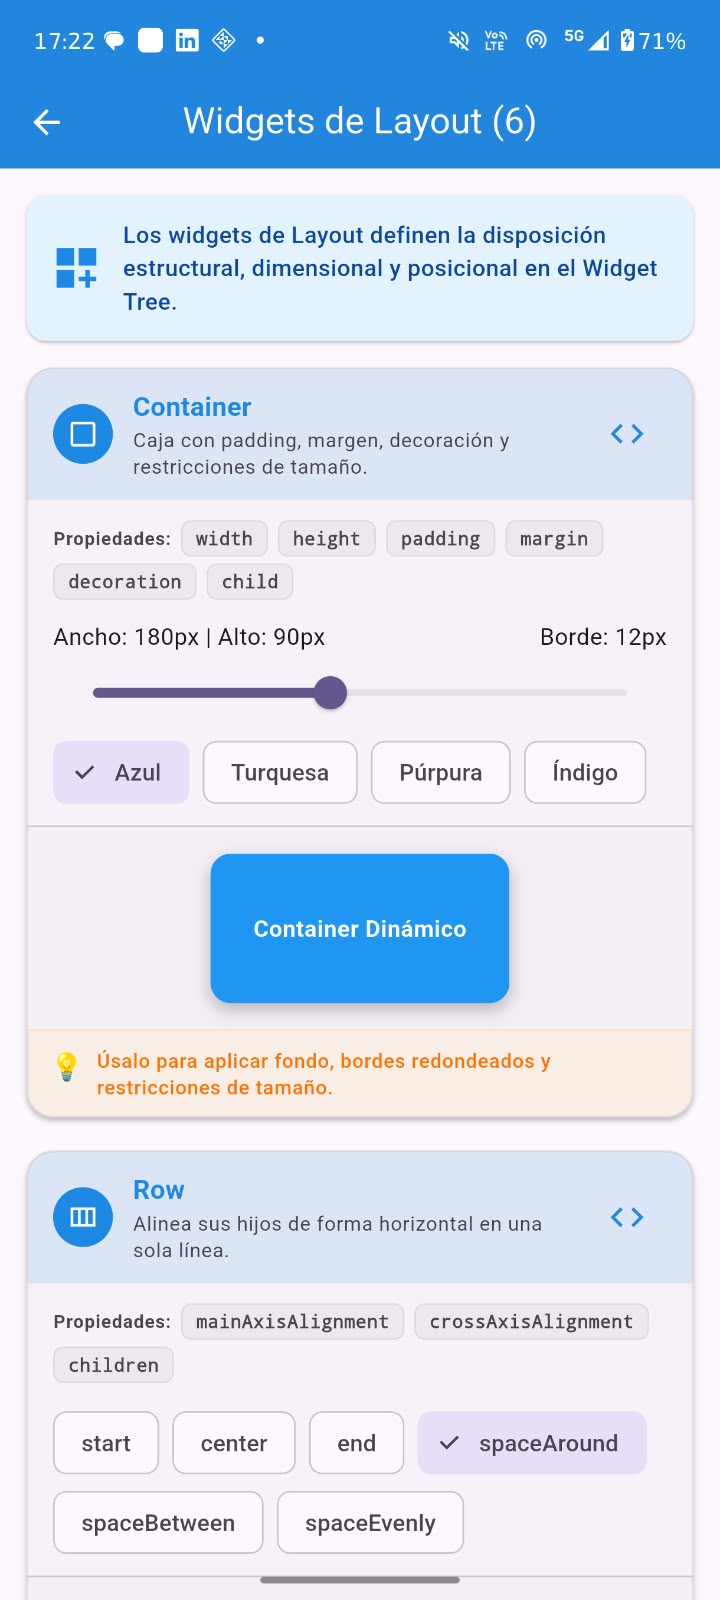
\includegraphics[width=0.88\linewidth]{imagenes/layout.png}
        \caption{Categoría Layout en ejecución móvil.}
        \label{fig:layout}
    \end{minipage}\hfill
    \begin{minipage}{0.48\textwidth}
        \centering
        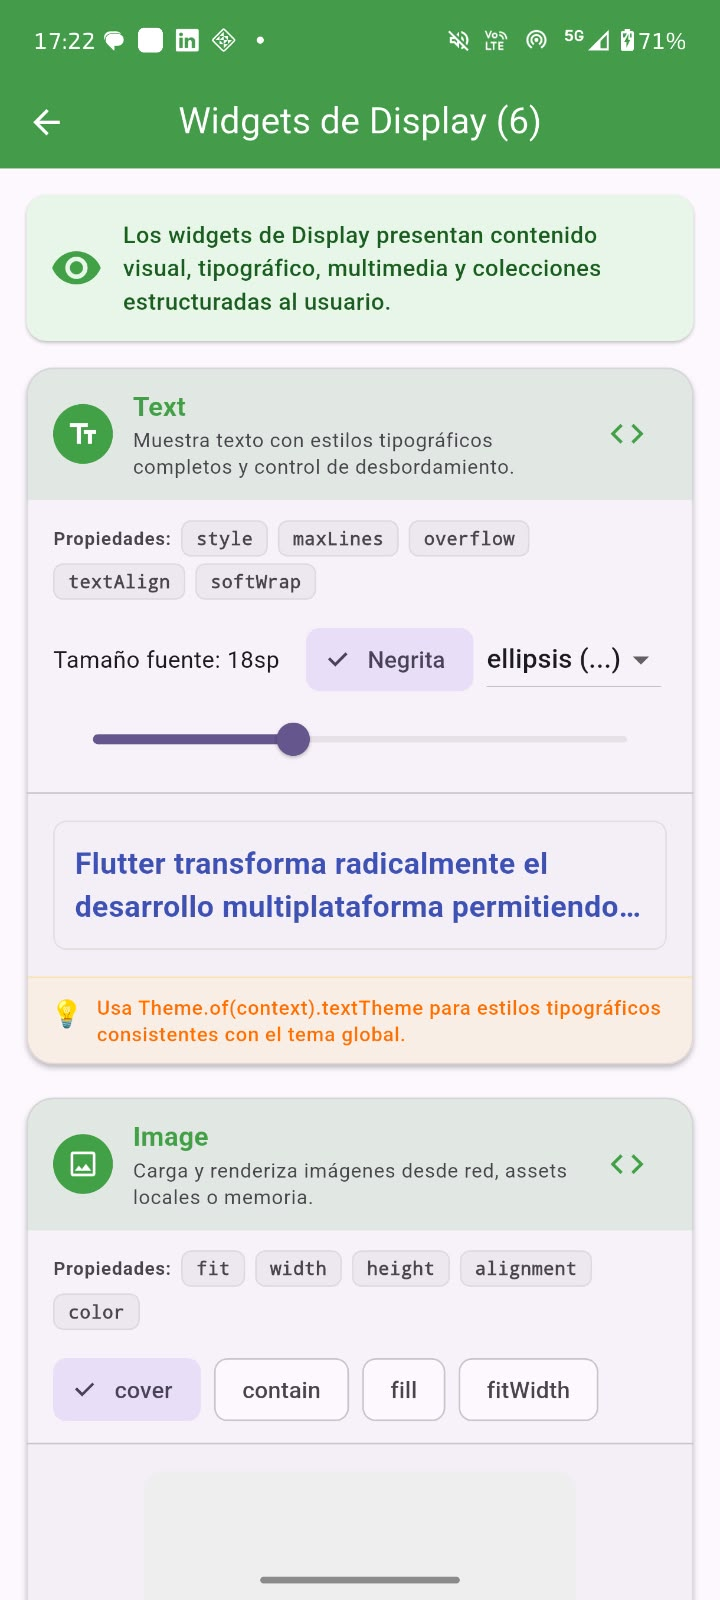
\includegraphics[width=0.88\linewidth]{imagenes/display.png}
        \caption{Categoría Display en ejecución móvil.}
        \label{fig:display}
    \end{minipage}
\end{figure}

\subsection{Categorías 3 y 4: Input y Navegación}
En la Figura~\ref{fig:input} se constata la captura de entrada de usuario mediante los controles interactivos de la categoría \textit{Input}: botones primarios (\texttt{ElevatedButton}), campos editables (\texttt{TextField}), controles booleanos (\texttt{Switch} y \texttt{Checkbox}), menú desplegable (\texttt{DropdownButton}) y control de rango (\texttt{Slider}). En la Figura~\ref{fig:navegacion} se observa la orquestación del flujo de navegación (\textit{Navegación}) mediante la barra superior (\texttt{AppBar}), la barra inferior de destinos (\texttt{BottomNavigationBar}), pestañas sincronizadas (\texttt{TabBar/TabBarView}) y la pila de rutas (\texttt{Navigator}).

\begin{figure}[htbp]
    \centering
    \begin{minipage}{0.48\textwidth}
        \centering
        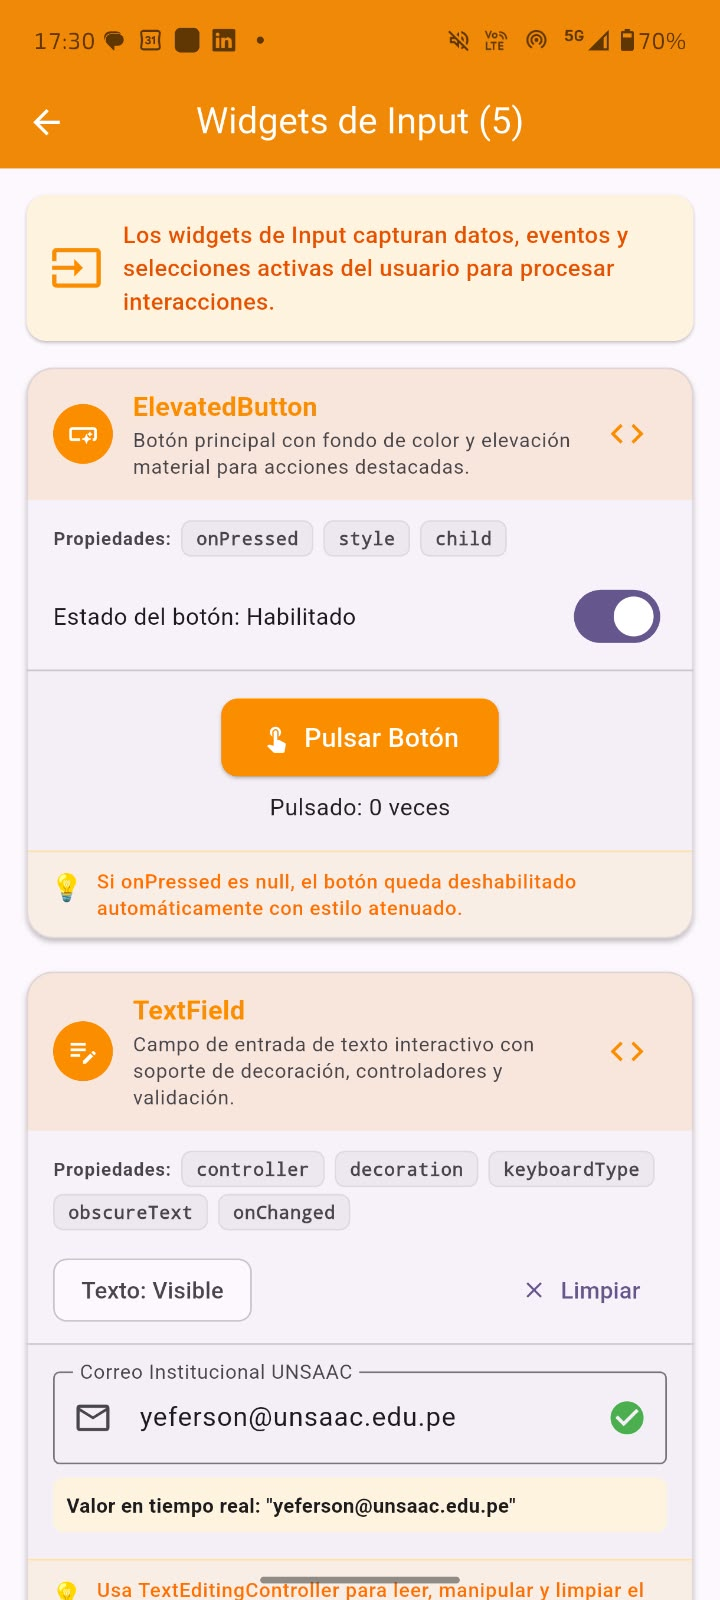
\includegraphics[width=0.88\linewidth]{imagenes/input.jpeg}
        \caption{Categoría Input en ejecución móvil.}
        \label{fig:input}
    \end{minipage}\hfill
    \begin{minipage}{0.48\textwidth}
        \centering
        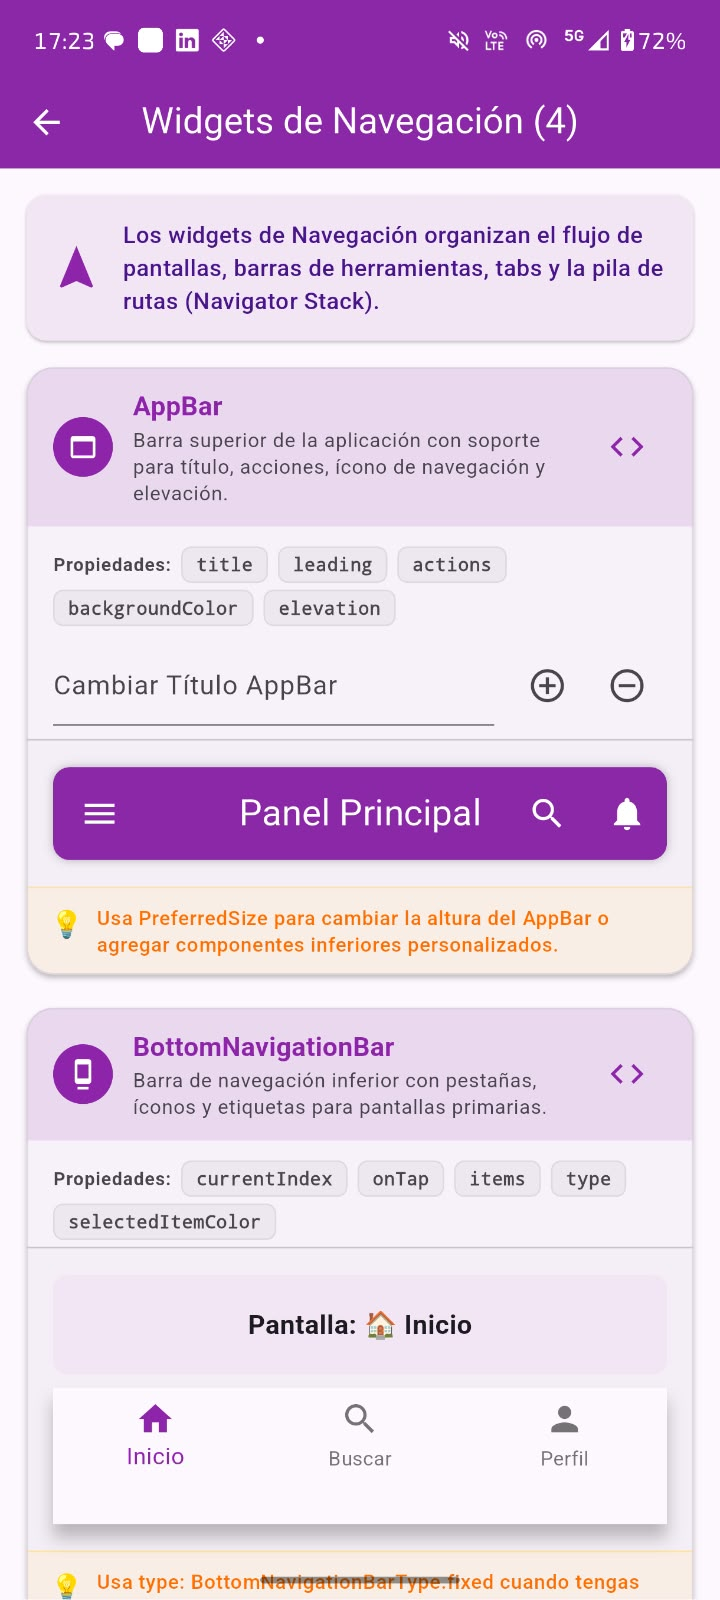
\includegraphics[width=0.88\linewidth]{imagenes/navegacion.png}
        \caption{Categoría Navegación en ejecución móvil.}
        \label{fig:navegacion}
    \end{minipage}
\end{figure}

\subsection{Categoría 5: Feedback y Notificaciones del Sistema}
En la Figura~\ref{fig:feedback} se exhiben los componentes de la categoría \textit{Feedback}: emisión de notificaciones flotantes (\texttt{SnackBar}), diálogos modales de decisión (\texttt{AlertDialog}), etiquetas con borrado y selección contextual (\texttt{Chip/FilterChip}), e indicadores circulares y lineales con animación de carga continua y simulación en tiempo real (\texttt{CircularProgressIndicator} y \texttt{LinearProgressIndicator}).

\begin{figure}[htbp]
    \centering
    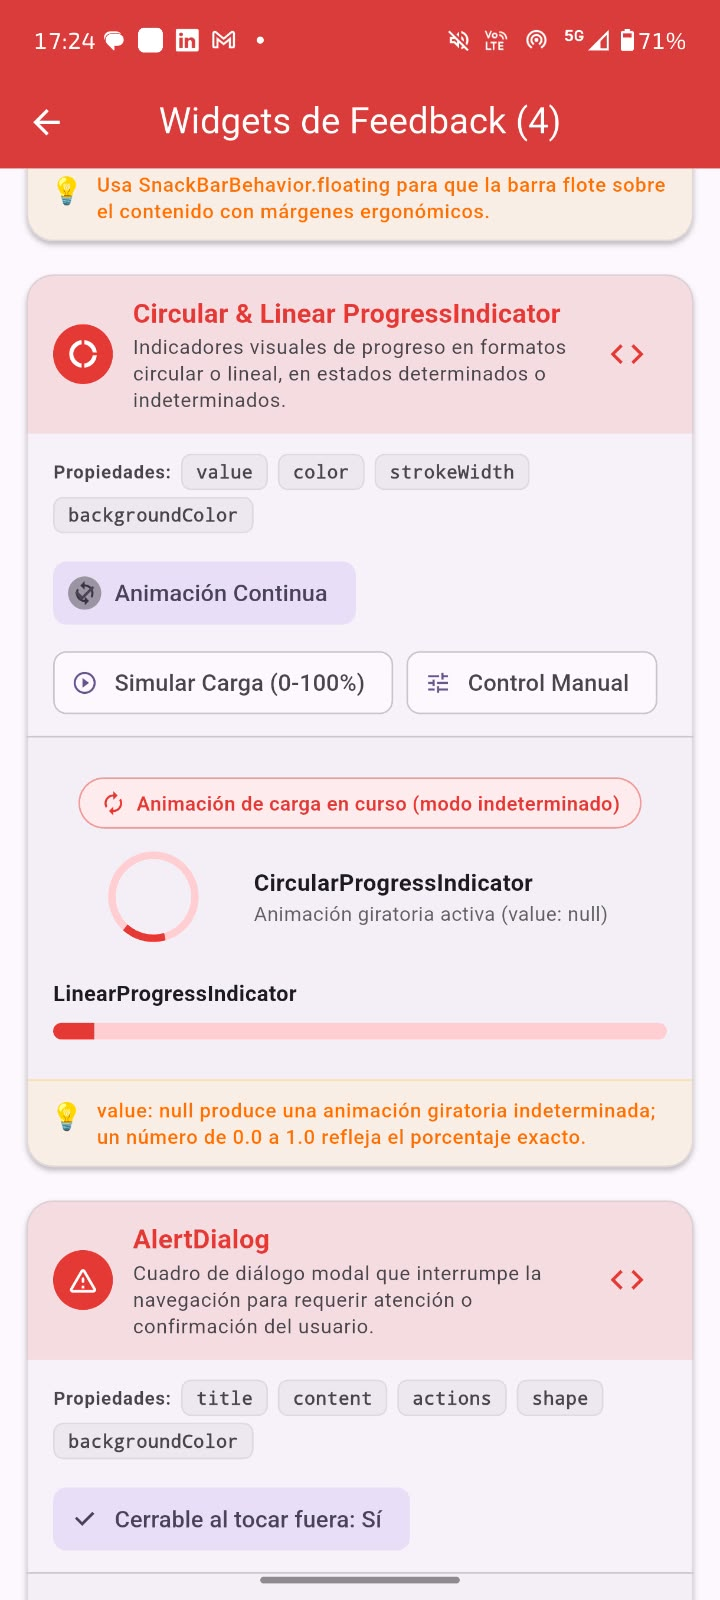
\includegraphics[width=0.48\linewidth]{imagenes/feedback.png}
    \caption{Categoría Feedback y Notificaciones en ejecución móvil.}
    \label{fig:feedback}
    \vspace{0.3cm}
\end{figure}

% ==============================================================================
% 8. DECÁLOGO DE BUENAS PRÁCTICAS EN FLUTTER
% ==============================================================================
\section{Decálogo de Buenas Prácticas de Ingeniería en Flutter}

\begin{enumerate}[leftmargin=*]
    \item \textbf{Todo en Flutter es un Widget:} Desde el elemento visual más minúsculo hasta el contenedor global \texttt{MaterialApp}.
    \item \textbf{Inmutabilidad con \texttt{const}:} Al marcar widgets con constructores constantes, Flutter reutiliza la instancia en memoria y evita reconstruir ramas completas del árbol de widgets.
    \item \textbf{Preferencia de \texttt{StatelessWidget}:} Reduce la complejidad cognitiva y el uso de memoria; emplea \texttt{StatefulWidget} únicamente cuando el widget requiera mutar su propio estado.
    \item \textbf{Gestión de Estado Reactiva y Desacoplada:} En proyectos medianos o grandes, separar la lógica de negocio de la vista usando patrones como Riverpod, BLoC o Provider.
    \item \textbf{Aprovechamiento del Widget Inspector:} DevTools permite inspeccionar el diseño en tiempo real, visualizar cajas delimitadoras (\textit{bounding boxes}) y diagnosticar desbordamientos (\textit{RenderFlex overflow}).
    \item \textbf{Agilidad con Hot Reload y Hot Restart:} \textit{Hot Reload} inyecta el código compilado en la máquina virtual Dart preservando el estado en milisegundos; \textit{Hot Restart} reinicia la máquina virtual para reconstruir estados iniciales.
    \item \textbf{Principio DRY y Extracción de Clases:} Extraer bloques de widgets en clases separadas (\texttt{StatelessWidget}) en lugar de funciones auxiliares (\texttt{Widget _buildItem()}), asegurando que el framework optimice las reconstrucciones locales.
    \item \textbf{Diseño Adaptativo con \texttt{MediaQuery}:} Utilizar \texttt{MediaQuery.of(context).size} e \textit{insets} para adaptar el layout dinámicamente a teléfonos, tabletas y monitores.
    \item \textbf{Ajuste Armónico con \texttt{FittedBox}:} Escalar elementos para que encajen dentro de su caja contenedora sin romper las restricciones de diseño.
    \item \textbf{Sistema de Diseño Coherente con \texttt{ColorScheme}:} Diseñar con colores semánticos (\texttt{colorScheme.primary}, \texttt{colorScheme.surface}) para que la aplicación responda de forma automática al modo oscuro del sistema.
\end{enumerate}

% ==============================================================================
% 9. CONCLUSIONES
% ==============================================================================
\section{Conclusiones}

\begin{itemize}[leftmargin=*]
    \item La arquitectura de Flutter basada en widgets declarativos inmutables y la separación en tres árboles (\textit{Widget}, \textit{Element} y \textit{RenderObject}) permite un rendimiento óptimo al minimizar el repintado innecesario de la pantalla.
    \item Los 25 widgets analizados abarcan todas las dimensiones necesarias para construir interfaces móviles profesionales, desde la distribución espacial y la tipografía hasta la captura de eventos, navegación estructurada y retroalimentación al usuario.
    \item La implementación de un catálogo interactivo con componentes desacoplados como \texttt{WidgetDemoCard} proporciona un marco de aprendizaje práctico para comprender el impacto visual de cada propiedad en tiempo real.
    \item La ejecución exitosa de pruebas automatizadas con \texttt{flutter test} valida que la arquitectura es robusta, mantenible y libre de regresiones.
\end{itemize}

% ==============================================================================
% 10. REFERENCIAS BIBLIOGRÁFICAS
% ==============================================================================
\section{Referencias Bibliográficas}

\begin{enumerate}[leftmargin=*]
    \item Flutter Team. \textit{Flutter Architectural Overview}. Google LLC, 2026. Disponible en: \url{https://docs.flutter.dev/resources/architectural-overview}.
    \item Google Material Design. \textit{Material 3 Design Specifications}. Google LLC, 2026. Disponible en: \url{https://m3.material.io}.
    \item Windmill, Eric. \textit{Flutter in Action}. Manning Publications, 2020.
    \item Ccacyahuillca Bejar, Hans Harley. \textit{Guía de Prácticas: Desarrollo de Software II}. Universidad Nacional de San Antonio Abad del Cusco (UNSAAC), 2026.
\end{enumerate}

\end{document}
